\section{LF04 - Digitaltechnik}
%

\subsection{tl;dr - Zusammenfassung der Zusammenfassung}
ASCII
Schaltalgebra leitet sich aus der Boolschen Logik ab.


%%% Ende: tl;dr

\subsection{Zahlensysteme}

\paragraph{Umrechnung von Binär- in Hexadezimal- und Dezimal-Systemen}~\\
\paragraph{Binäre Darstellung von negativen Zahlen}~\\
%%% Ende: Zahlensysteme

\subsection{Codes - ASCII}

Es gibt vom ASCII mehrere Abwandlungen, bei der einige wenig genutzte Zeichen durch regionale Sonderzeichen ersetzt werden. Beispielsweise handelt es sich bei ISO 636 (DIN 66003) um eine deutsche ASCII-Codierung, die auch Umlaute enthält. Zunächst wurde ASCII in 7-Bit kodiert. Später dann in 8-Bit\footnote{{\url http://www.ascii-code.com/}}, da mit 7-Bit nicht genug Sondereichen kodiert werden konnten und so das Problem entstand, dass US-ASCII \verb+{ a[i] = '\n'; }+ unter DE-ASCII als \verb+ä aÄiÜ = 'Ön'; ü+ ausgegeben wurde. 7-Bit ASCII wurde nicht ersetzt, sondern erweitert. Durch die 8-Bit kodieren sind insgesamt 256 Zeichen möglich. Die ersten $32$ sind sogenannte Steuerzeichen. Die folgenden $96$ sind die druckbaren Zeichen. Die letzten $128$ Zeichen enthalten die zusätzlichen Zeichen, bspw. \euro.\\

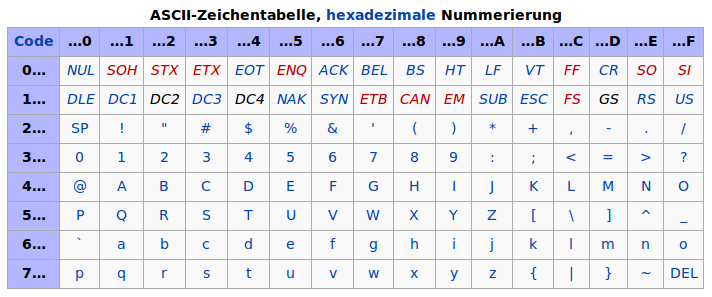
\includegraphics[scale=0.4]{1jahr_pictures/lf04-pic/lf04-7bit-ascii-hex.png}

ASCII-Protokolle nennt man Netzwerkprotokolle, welche ausschließlich mittels menschen-lesbarer Wörter oder zumindest ausschließlich mittels menschen-lesbarer Zeichen aus dem ASCII-Zeichensatz kommunizieren. ASCII-Protokolle sind zum Beispiel POP3, SMTP, HTTP, FTP und IRC.
%%% Ende: Codes

\subsection{Schaltalgebra}
Die Schaltalgebra geht aus der Boolschen Logik hervor. Die Variablen $A$, $B$ und $C$ können jeweils $1$ oder $0$ annehmen.

Das Ergebnis einer $UND$-Operation ist negativ, sobald nur ein Element den Wert $0$ hat.
\begin{tabular}{l|l|l}
	$A$	& $B$	& {$A$ \wedge $B$}\\
	1	& 1		& 1 \\
	1	& 0		& 0 \\
	0	& 1		& 0 \\
	0	& 0		& 0 \\
\end{tabular}

Damit das Ergebnis einer $ODER$-Operation $0$ ist, müssen beide Elemente den Wert $0$ haben. In den andern Fällen ist das Ergebnis $1$.
\begin{tabular}{l|l|l}
	$A$	& $B$	& {$A$ \vee $B$}\\
	1	& 1		& 1 \\
	1	& 0		& 1 \\
	0	& 1		& 1 \\
	0	& 0		& 0 \\
\end{tabular}

In der Logik wird eine $ODER$-Operation kontraintuitiv definiert. Dem natursprachlichen \ql oder\qr\ entspricht das $XOR$ (eXclusive OR; dt. entweder oder).
\begin{tabular}{l|l|l}
	$A$	& $B$	& {$A$ \veebar $B$}\\
	1	& 1		& 0 \\
	1	& 0		& 1 \\
	0	& 1		& 1 \\
	0	& 0		& 0 \\
\end{tabular}
%%% Ende: Schaltalgebra

\subsection{Digitale Rechenschaltungen}

Einige Rechenschaltungen der Digitaltechnik
\begin{itemize}
	\item Addiererschaltungen
	\item Subtrahiererschaltungen
	\item Addier-Subtrahier-Werke
	\item Multiplikationsschaltungen
	\item Arithmetisch-logische Einheit (ALU)
\end{itemize}

Halbaddierer
Volladdierer
3-Bit Volladdierer


%%% Ende: Digitale Rechenschaltungen